\documentclass[11pt,a4paper]{article}
\usepackage[margin=1in]{geometry}
\usepackage{amsmath}
\usepackage{algorithm}
\usepackage{algpseudocode}
\usepackage{hyperref}
\usepackage{graphicx}
\usepackage{float}

\title{Parallelization Report of Stock Prediction Pipeline}
\author{Nicola Rohner}

\begin{document}
\maketitle

\section{Parallelization Report}

\subsection{Implementation}
The parallelization of the stock analysis script was implemented using Dask. The key steps in the implementation were:
Setting up a Dask client, Creating a Dask bag from the list of files and Processing all files in parallel using Dask's map and compute functions.
This approach allows for file-level parallelization, where each file is processed independently and concurrently.
Note:
For example cross-validation is not parallelized, processes would compete for the same CPU threads. Nested parallelism typically leads to thread thrashing and overhead. Was more efficient to keep ETL parallel and cross-validation sequential within each worker

\subsection{Impact on Speed}
The parallelization improved the processing speed of the script, particularly when dealing with a large number of files. My test revealed:
A max. Speedup around 6.22x, performance gains were most noticeable with a higher number of processes.

\subsection{Reflection on the Development Process}
Dask's high-level API significantly simplified the parallelization process, allowing me to maintain much of the original code structure, especially if you code in a functional style.
The parallelized version demonstrated excellent scalability, on local multi-core machines.
For very small datasets or when processing only a few files, I found that the overhead of setting up the Dask infrastructure could outweigh the benefits of parallelization. 


\section{Function-by-Function Analysis}

\begin{enumerate}
    \item \textbf{load\_data(filename)}: $O(n)$
    \begin{itemize}
        \item This function primarily involves reading the CSV file, which scales linearly with the number of rows.
    \end{itemize}
    
    \item \textbf{add\_features(df)}: $O(n)$
    \begin{itemize}
        \item The rolling window operations (MA5, MA20, LR\_Slope, RSI) and the exponential moving average (EMA) calculations for MACD all have mostly linear time complexity.
    \end{itemize}
    
    \item \textbf{feature\_selection(df)}: $O(n \cdot f)$, where $f$ is the number of features
    \begin{itemize}
        \item The SelectKBest with f\_regression algorithm has a time complexity of $O(n \cdot f)$.
    \end{itemize}
    
    \item \textbf{train\_models(df)}: $O(k \cdot n^2 \cdot m)$, where $k$ is the number of cross-validation folds, $n$ is the number of samples, and $m$ is the number of features
    This function's complexity is dominated by the cross-validation of the SVR model with RBF kernel.
    \begin{itemize}
        \item RandomForestRegressor: $O(n_{\text{trees}} \cdot n \cdot \log(n) \cdot m)$
        \item LinearRegression: $O(n \cdot m^2)$
        \item SVR (RBF kernel): $O(n^2 \cdot m)$
        \item Cross-validation multiplies each model's complexity by $k$ (number of folds)
    \end{itemize}

    \item \textbf{process\_file(filename)}: $O(k \cdot n^2 \cdot m)$, where $k$ is the number of cross-validation folds, $n$ is the number of samples, and $m$ is the number of features
    \begin{itemize}
        \item load\_data(filename): $O(n)$, where $n$ is the number of rows in the file
        \item add\_features(df): $O(n)$
        \item feature\_selection(df): $O(n \cdot m)$
        \item train\_models(df): $O(k \cdot n^2 \cdot m)$ - dominates the overall complexity
        \item File operations (os.makedirs, joblib.dump): $O(1)$ relative to data processing
        \item The overall complexity is determined by the most computationally expensive operation, train\_models
    \end{itemize}

    \item \textbf{Overall Script Complexity}: $O(F \cdot k \cdot n^2 \cdot m)$
    \begin{itemize}
        \item $F$: Total number of files to process
        \item $k$: Number of cross-validation folds
        \item $n$: Number of samples in the largest file
        \item $m$: Number of features
    \end{itemize}
    \begin{itemize}
        \item File listing operations: $O(F)$
        \item Dask bag creation: $O(F)$
        \item The dominant factor is the parallel execution of process\_file for each file
    \end{itemize}
\end{enumerate}

\subsection{Machine Learning Algorithms}
A more detailed look at the time complexities of the machine learning algorithms used:

\begin{itemize}
    \item \textbf{Linear Regression}
    \begin{itemize}
        \item Training: $O(nm^2)$
        \item Prediction: $O(m)$
        \item Generally fast for both training and prediction, especially when the number of features $(m)$ is relatively small.
    \end{itemize}
    
    \item \textbf{Support Vector Regression (SVR)}
    \begin{itemize}
        \item Training: $O(n^2m)$
        \item Prediction: $O(vm)$, where $v$ is the number of support vectors
        \item Potentially the slowest algorithm, especially for large datasets.
    \end{itemize}
    
    \item \textbf{Random Forest Regressor}
    \begin{itemize}
        \item Training: $O(t \cdot u \cdot n \log n)$, where $u$ is the number of features considered for splitting
        \item Prediction: $O(t \log n)$
        \item Generally efficient, especially when the number of trees $(t)$ and features considered for splitting $(u)$ are not too large.
    \end{itemize}
\end{itemize}

\section{Comparison and Analysis}

\subsection{Theoretical Complexity}
Sequential version: $O(F \cdot k \cdot n^2 \cdot m)$

Where:
\begin{itemize}
    \item $F$: Total number of files
    \item $k$: Number of cross-validation folds
    \item $n$: Number of samples in the largest file
    \item $m$: Number of features
\end{itemize}

\subsection{Experiments}
The runtimes of the parallelized version looks as follows:

Settings for the runs:
\begin{itemize}
    \item 1 process: $n\_workers = 1$ and $n\_threads = 1$
    \item 2 processes: $n\_workers = 2$ and $n\_threads = 1$
    \item 4 processes: $n\_workers = 2$ and $n\_threads = 2$
    \item 9 processes: $n\_workers = 3$ and $n\_threads = 3$
    \item 16 processes: $n\_workers = 4$ and $n\_threads = 4$
    
\end{itemize}

\begin{figure}[H]
    \centering
    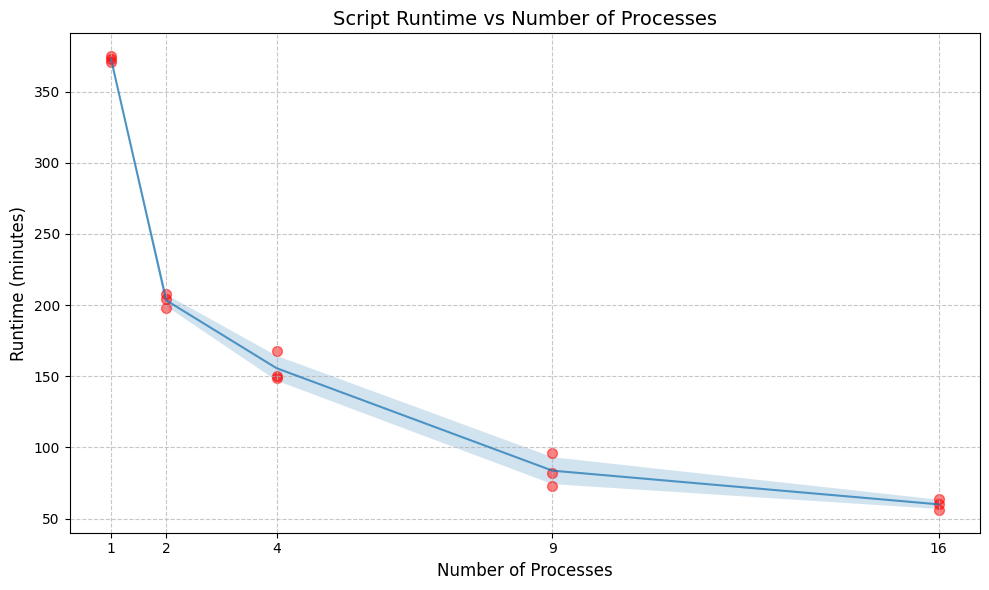
\includegraphics[width=0.8\textwidth]{runtime.png}
    \caption{Speedup of Parallelized Stock Prediction Pipeline}
\end{figure}

The speedup shows strong initial gains when adding the first few processes, but flattens after 9 processes. This could be due communication overhead between processes becoming significant, and resource contention as processes compete for CPU/memory.
The experiment was run on a machine with the following CPU:\newline
$11th Gen Intel(R) Core(TM) i9-11900K @ 3.50GHz, 3504 MHz, 8 Cores, 16 Logical Processors$.
\newline \newline
For this experiment, the number of files was varied from 1 to 8539, and the processing time was measured for each configuration.
Configurations: $n\_workers = 1, n\_threads = 1$

\begin{figure}[H]
    \centering
    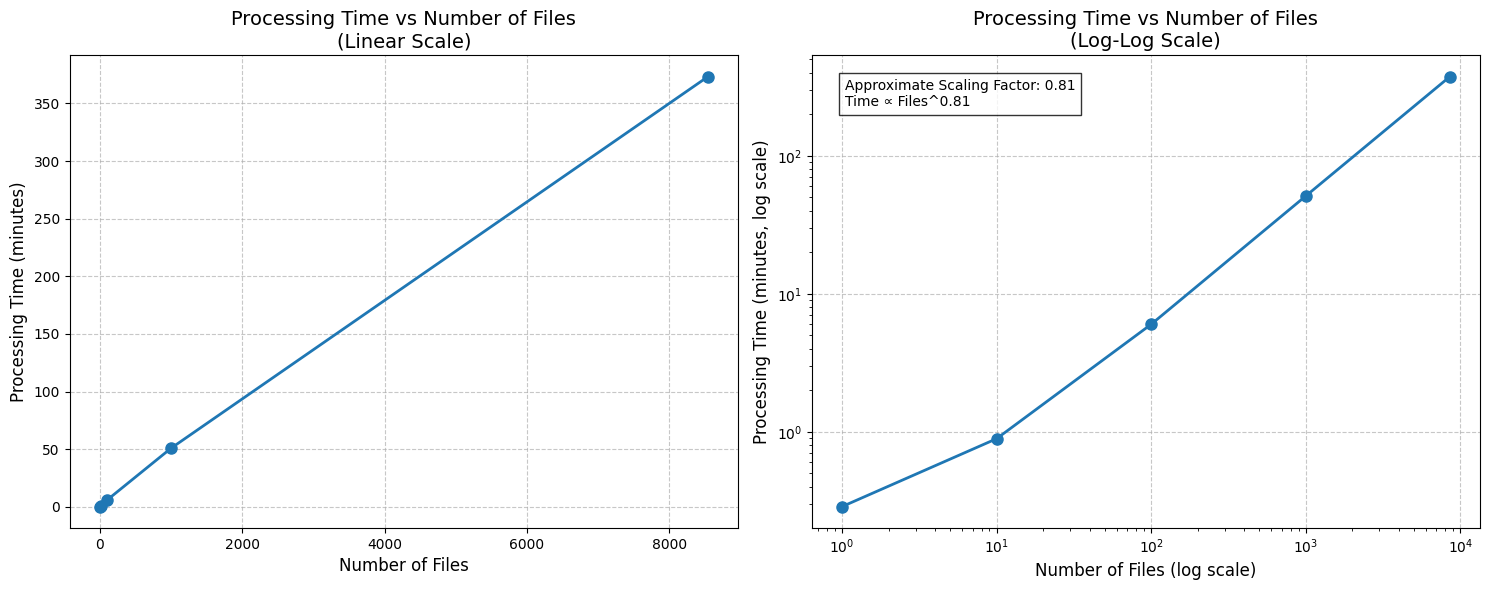
\includegraphics[width=0.8\textwidth]{runtime2.png}
    \caption{Processing Time vs Number of Files}
\end{figure}

Looking at the plots, we can see that with 1 worker and 1 thread:
\begin{enumerate}
    \item The processing time increases predictably as files increase (from 1 to 10,000 files)
    \item The relationship between files and time shows a mostly linear trend in the left plot
    \item The log-log scale (right plot) reveals a scaling factor of 0.81, showing the relationship between files and processing time
\end{enumerate}

\subsection{Analysis}

\[ \text{Speedup}_{\text{overall}} = \frac{1}{(1-p) + \frac{p}{n}} \]

For example, with our 16 processes case:
\[ \text{Speedup}(16) = \frac{373 \text{ min}}{60 \text{ min}} = 6.22\times \]

Using this observed speedup, we can determine the parallelizable portion $p$:
\[ 6.22 = \frac{1}{(1-p) + \frac{p}{16}} \]
\[ p \approx 0.90 \text{ or } 90\% \text{ parallelizable} \]

Substituting back into Amdahl's formula:
\[ \text{Speedup}(n) = \frac{1}{(1-0.90) + \frac{0.90}{n}} = \frac{1}{0.1 + \frac{0.90}{n}} \]


The speedup is bounded to Amdahl's Law, which limits the maximum speedup achievable by parallelization.
Which in my case is around 10x, as the parallelizable portion is 90\%.

\begin{figure}[H]
    \centering
    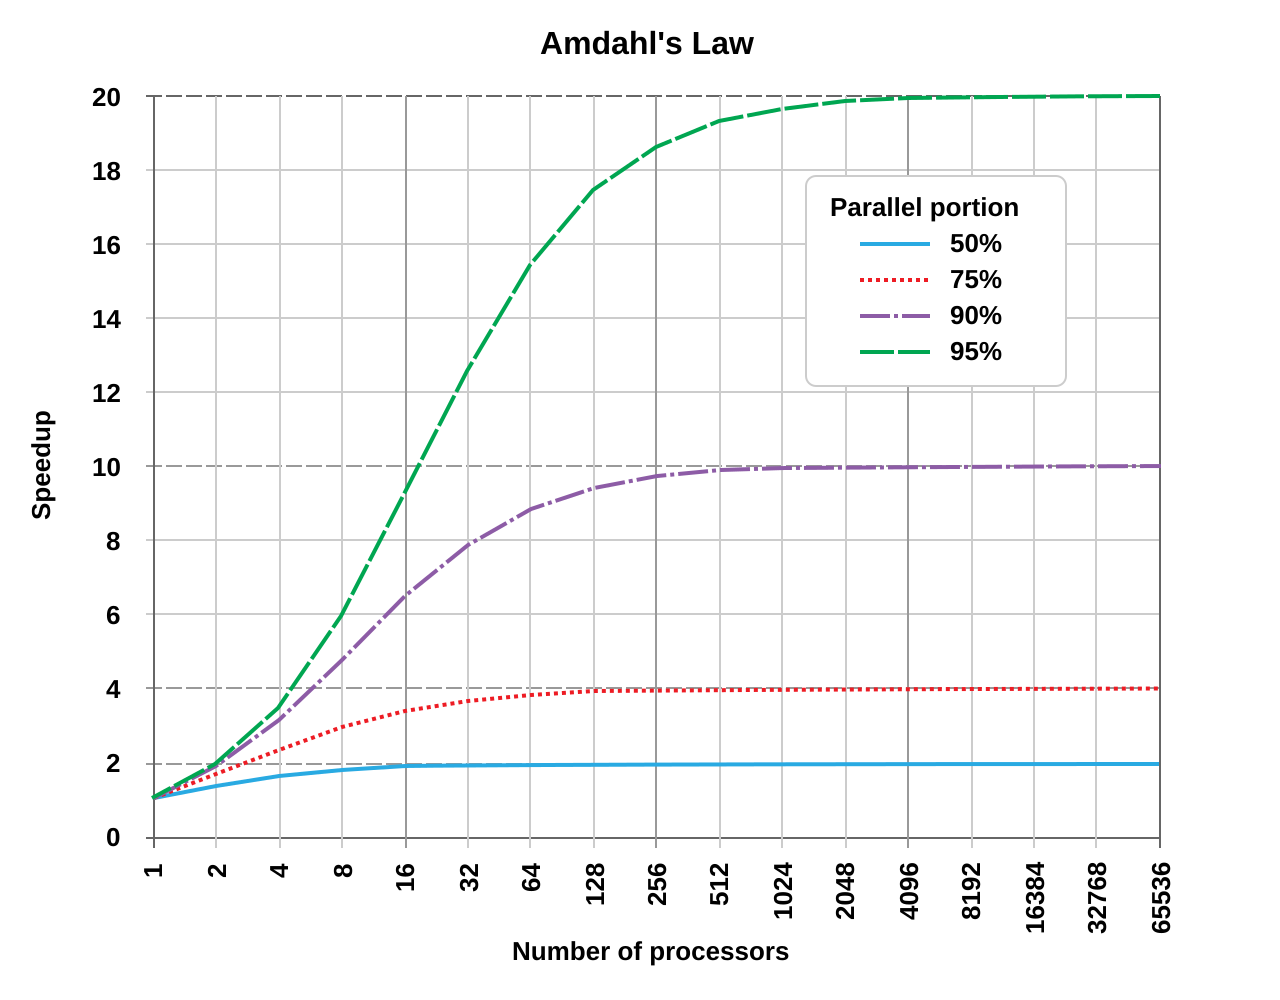
\includegraphics[width=0.8\textwidth]{amdahl.png}
    \caption{Amdahl's Law: Speedup vs Number of Processes}
\end{figure}

\section{Sources}
\begin{enumerate}
    \item Virgolin, M. (2021). Time complexity for different machine learning algorithms.\url{https://marcovirgolin.github.io/extras/details_time_complexity_machine_learning_algorithms/}
    \item Dask Development Team. Dask Documentation.  \url{https://docs.dask.org/en/stable/}
    \item Amdahl's Law. \url{https://en.wikipedia.org/wiki/Amdahl%27s_law}
\end{enumerate}

\end{document}